
\chapter{Referencial Teórico}

\section{Circuitos Digitais}

CPU

\subsection{Linguagem de Descrição de \textit{Hardware}}

CPU

\subsection{Arranjo de Portas Programável em Campo}

CPU

\subsection{Circuitos Sequenciais}

CPU

\subsection{Lógica Booleana e Circuitos Combinacionais}

CPU

\section{Organização e Arquitetura de Computadores}

CPU

\subsection{Arquitetura de Processadores Digitais}

CPU

\subsection{Controladores de Dispositivos Externos}

CPU

\section{Sistemas Operacionais}

CPU

\section{\textit{Software} Básico}

CPU

\subsection{Carregadores}

CPU

\subsection{Ligadores}

Após arquivos objeto de um ou vários módulos de compilação serem gerados por um montador, é preciso combiná-los em um único arquivo que pode ser carregado para a memória por um programa carregador do sistema operacional.

\subsection{Montadores}

Montadores são programas que traduzem um módulo de compilação em linguagem \textit{assembly} para uma versão em linguagem de máquina. O armazenamento desta versão é feito em um arquivo objeto. Como veremos em uma seção adiante, um arquivo objeto é uma versão binária de um módulo de compilação, que geralmente fica a um passo de poder ser carregada para execução.

\subsection{Linguagem de máquina}

Anteriormente vimos que uma linguagem de montagem, ou linguagem \textit{assembly}, é formada por símbolos mnemônicos, ou palavras-chave, que identificam as instruções que um processador é capaz de executar.

A etapa seguinte à compilação é a montagem. Nesta etapa, é necessário traduzir os mnemônicos \textit{assembly} para sequências de \textit{bits}. Um \textit{bit} é um dígito que pode assumir apenas o valor 0 (zero) ou o valor 1 (um). Durante a execução de um programa, estas sequências de \textit{bits} serão diretamente interpretadas por uma \textit{CPU}.

Costuma-se dizer que a etapa de montagem é onde está localizada a interface \textit{software}-\textit{hardware}. Uma \textit{ISA} - \textit{Instruction Set Architecture}, ou Arquitetura de Conjunto de Instruções - é uma especificação das instruções que uma implementação de processador digital deve fornecer. Esta especificação, entre outras coisas, estabelece os formatos que as sequências de \textit{bits} geradas por montadores devem seguir. Este é o principal conhecimento necessário para construir um montador.

\begin{figure}[ptb]
  \begin{center}
    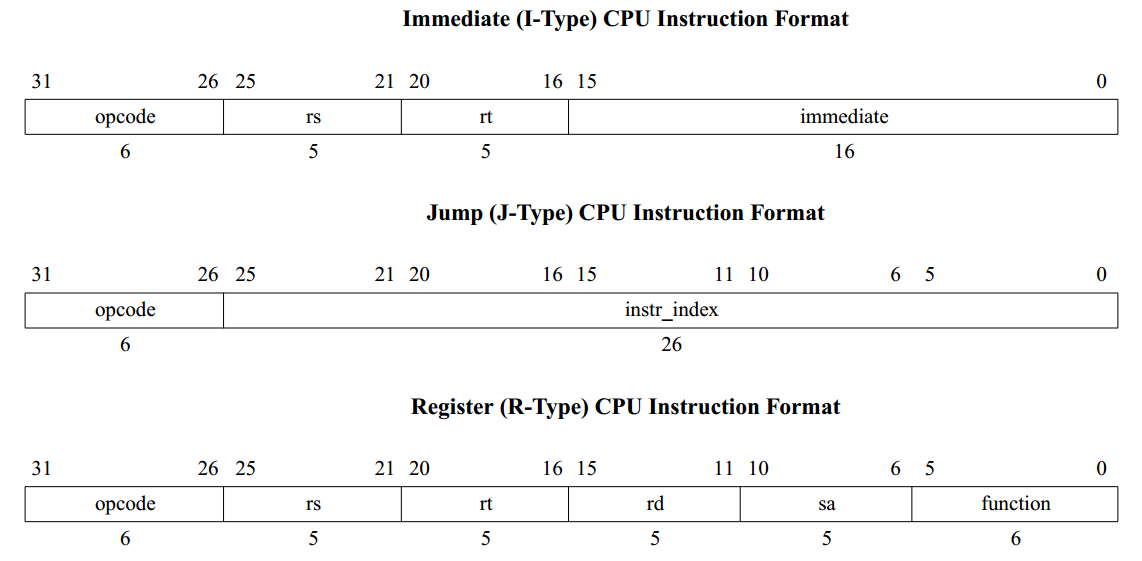
\includegraphics[scale=.45]{imagens/instrucoes_mips}
  \end{center}
  \caption{Os três formatos principais da \textit{ISA} \textit{MIPS32}.}
  \label{instrucoes_mips}
\end{figure}

A figura \ref{instrucoes_mips} mostra os três formatos principais de instruções da arquitetura \textit{RISC} \textit{MIPS32}. Grandes quantidades de instruções se encaixam em cada um dos três formatos. Nesta arquitetura, toda e qualquer instrução ocupa uma palavra de 32 \textit{bits}.

A figura \ref{instrucoes_ia32} mostra o formato geral para uma instrução qualquer da arquitetura \textit{CISC} \textit{IA-32}, criada pela Intel. Nesta arquitetura, o tamanho das instruções vai de 1 até 17 \textit{bytes} (um \textit{byte} são exatamente 8 \textit{bits}).

Com o conhecimento de como cada mnemônico deve ser convertido para código de máquina, podemos construir um montador para uma determinada arquitetura de processadores. À seguir descrevemos os algoritmos clássicos de montagem.

\begin{figure}[ptb]
  \begin{center}
    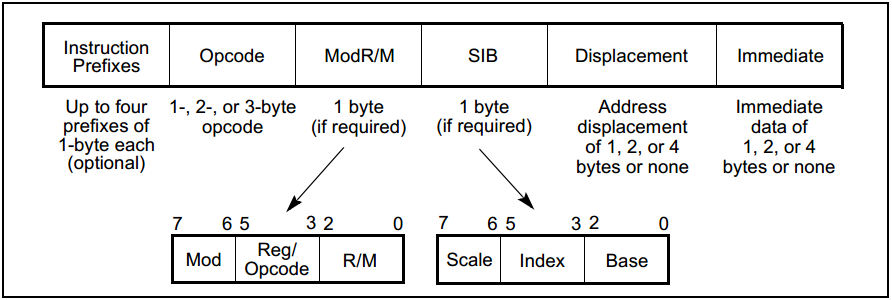
\includegraphics[scale=.6]{imagens/instrucoes_ia32}
  \end{center}
  \caption{Formato geral de uma instrução da \textit{ISA} \textit{IA-32}.}
  \label{instrucoes_ia32}
\end{figure}

\subsection{Algoritmos de montagem}

O problema da montagem pode ser colocado da seguinte forma: um módulo de compilação em linguagem \textit{assembly} contém dados e instruções mnemônicas que devem ser convertidas para binário seguindo a ordem em que aparecem. Para termos a noção de localização de um dado ou instrução, temos o conceito de endereço de memória.

Antes de definirmos o conceito de endereço de memória, precisamos definir o conceito de palavra. Uma palavra é um agrupamento de uma quantidade fixa de \textit{bits}. Uma \textit{ISA} determina os diferentes tamanhos de palavras que podem ser utilizados para escrever um programa. Geralmente, o menor tamanho de palavra suportado é o \textit{byte}, enquanto os outros tamanhos costumam ser múltiplos em potência de 2 de um \textit{byte}.

Aqui iremos nos referir a um endereço de memória como um número cuja unidade é o menor tamanho de palavra definido por uma arquitetura. Para referenciar endereços, linguagens de montagem costumam utilizar o que chamamos de símbolo, ou rótulo. Um símbolo pode ser uma palavra ou uma frase de linguagem natural.

Para realizar a conversão de um arquivo \textit{assembly} para binário, é necessário que um algoritmo de montagem realize passagens no arquivo de entrada, coletando informações de montagem. Com informação suficiente, o montador é capaz de colocar os dados em determinados endereços, colocar as instruções na ordem em que aparecem em outros endereços e substituir ocorrências de rótulos por seus respectivos endereços.

A próxima subseção descreve o algoritmo de duas passagens, o mais trivial.

\subsection{O algoritmo de duas passagens}

Na primeira passagem pelo código \textit{assembly}, este algoritmo cria uma tabela de símbolos.

A tabela de símbolos é uma estrutura indexada por símbolos (ou rótulos). Para cada símbolo que indexar a tabela, temos uma entrada com o endereço ao qual o símbolo se refere e algumas informações adicionais. É criada uma entrada nesta tabela para cada rótulo que for encontrado no código-fonte. Rótulos podem ser criados tanto para dados, quanto para instruções.

Em um programa \textit{assembly}, símbolos podem estar presentes tanto em definições de símbilos, ou seja, em locais onde o endereço de um símbolo é estabelecido, quanto podem estar contidos em instruções que referenciam endereços através de símbolos. Ao encontrar a definição de um símbolo, o montador pode gerar um erro, ou aviso, caso este símbolo já tenha sido definido anteriormente. Se a definição de um símbolo declara um dado, o montador pode colocar esta informação na entrada da tabela de símbolos.

Um montador tem a liberdade de implementar funcionalidades que facilitam a vida de um programador \textit{assembly}. Uma funcionalidade comumente implementada é a disponibilização de diretivas de pré-processamento. Diretivas são instruções ao próprio montador, ou seja, diretivas não são instruções que geram código de máquina.

Outra funcionalidade comum, é a utilização de pseudo-instruções. Pseudo-instruções utilizam mnemônicos e formatos parecidos com os das instruções concretas da \textit{ISA}, mas são instruções que não estão de fato implementadas em \textit{hardware}. É comum montadores fornecerem pseudo-instruções que expandem para muitas instruções concretas, que em conjunto realizam uma tarefa mais complexa.

Ainda na primeira passagem, o montador pode avaliar mnemônicos de instruções. Ao avaliar uma instrução, o montador pode gerar um erro caso não identifique o mnemônico da operação como válido. Um mnemônico válido pode ser o de uma instrução concreta, o de uma pseudo-instrução, ou pode ser uma diretiva de pré-processamento.

Com a tabela de símbolos pronta, o montador pode realizar a segunda passagem. Esta é a etapa em que o montador de fato gera código de máquina. 

O montador examina cada instrução à procura de símbolos. Símbolos que não estejam presentes na tabela de símbolos geram erro de montagem. Para instruções com símbolos definidos, o montador gera o código de máquina correspondente, substituindo cada símbolo por seu respectivo endereço.

Ao final da segunda passagem, o montador está pronto para gerar o arquivo objeto. Nesta etapa, coloca-se o código de máquina gerado junto com um espaço alocado para dados. Ao gerar de fato o arquivo de saída, o montador coloca nele informação de relocação, uma tabela de símbolos exportados e uma tabela de referências externas.

A figura \ref{duas_passagens} ilustra a execução de um algoritmo de duas passagens sobre um código \textit{assembly} hipotético (uma ref. aqui).

Voltaremos agora nossa atenção ao algoritmo de passagem única, desenvolvido para ser mais eficiente do que o algoritmo que acabamos de descrever. Iremos deixar a discussão sobre arquivos objeto para a subseção depois da próxima.

\begin{figure}[ptb]
  \begin{center}
    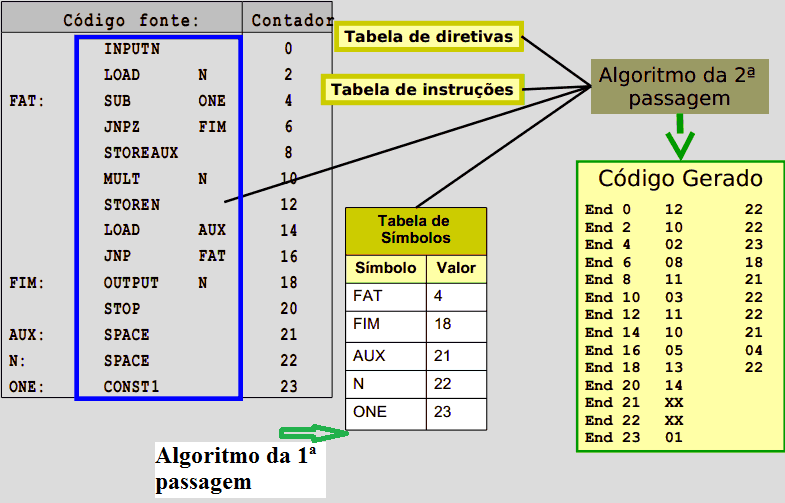
\includegraphics[scale=.7]{imagens/duas_passagens}
  \end{center}
  \caption{Ilustração do algoritmo de duas passagens sobre um \textit{assembly} hipotético.}
  \label{duas_passagens}
\end{figure}

\subsection{O algoritmo de passagem única}

Este algoritmo pode ser considerado uma evolução do algoritmo descrito acima.

Um montador de passagem única constrói a tabela de símbolos ao passo que gera código de máquina. Para trabalhar desta forma, são necessárias listas de referências pendentes.

Para cada símbolo encontrado em uma instrução que não estiver presente na tabela de símbolos, o algoritmo cria uma entrada na tabela, marca o símbolo como indefinido e cria uma lista de referências àquele símbolo.

Ao encontrar a definição de um símbolo, montadores de passagem única ainda geram erro, caso o símbolo já tenha sido definido anteriormente. No entanto, se o símbolo é encontrado na tabela, mas está marcado como indefinido, o algoritmo marca este símbolo como definido, estabelece seu endereço e itera sobre a lista de referências àquele símbolo atualizando os campos com o endereço válido. A implementação de um montador pode escolher atualizar as referências ao final da passagem, ao invés de realizar esta tarefa imediatamente.

Após a passagem ser realizada, se ainda existirem símbolos indefinidos o montador gera erro. O restante do processo é o mesmo que o descrito no algoritmo de duas passagens.

\subsection{Arquivos objeto}

Chamamos a saída de um montador de código objeto, ou arquivo objeto.

Tabela de relocação (endereços absolutos e relativos).

Tabela de símbolos exportados.

Tabela de referências externas.

\section{Compiladores}

CPU

\section{Criptografia}

CPU
